\clearpage
\setcounter{page}{1}
\maketitlesupplementary

\section{Details of Data Construction}
\subsection{Document Data Format}
As stated in Section~\ref{sec:data_engine}, documents in Doc-750K can be extracted in two formats: \textbf{Interleaved Text-Image Format} and rendered \textbf{Multi-Image Format}. The interleaved format utilizes an external PDF parser to extract text directly, avoiding OCR errors. However, this approach sacrifices some layout information. The multi-image format, commonly used in screenshot-based QA scenarios, preserves the complete layout but relies on the model's built-in OCR capabilities, which may introduce errors. Each format has its advantages and is suitable for different applications. By leveraging both formats, the model can develop complementary capabilities, enhancing its robustness across diverse input types. Examples of each format are shown in Figure~\ref{fig:multi-image} and Figure~\ref{fig:interleaved-image_text}, respectively.


\begin{figure*}[t]
    \centering
    {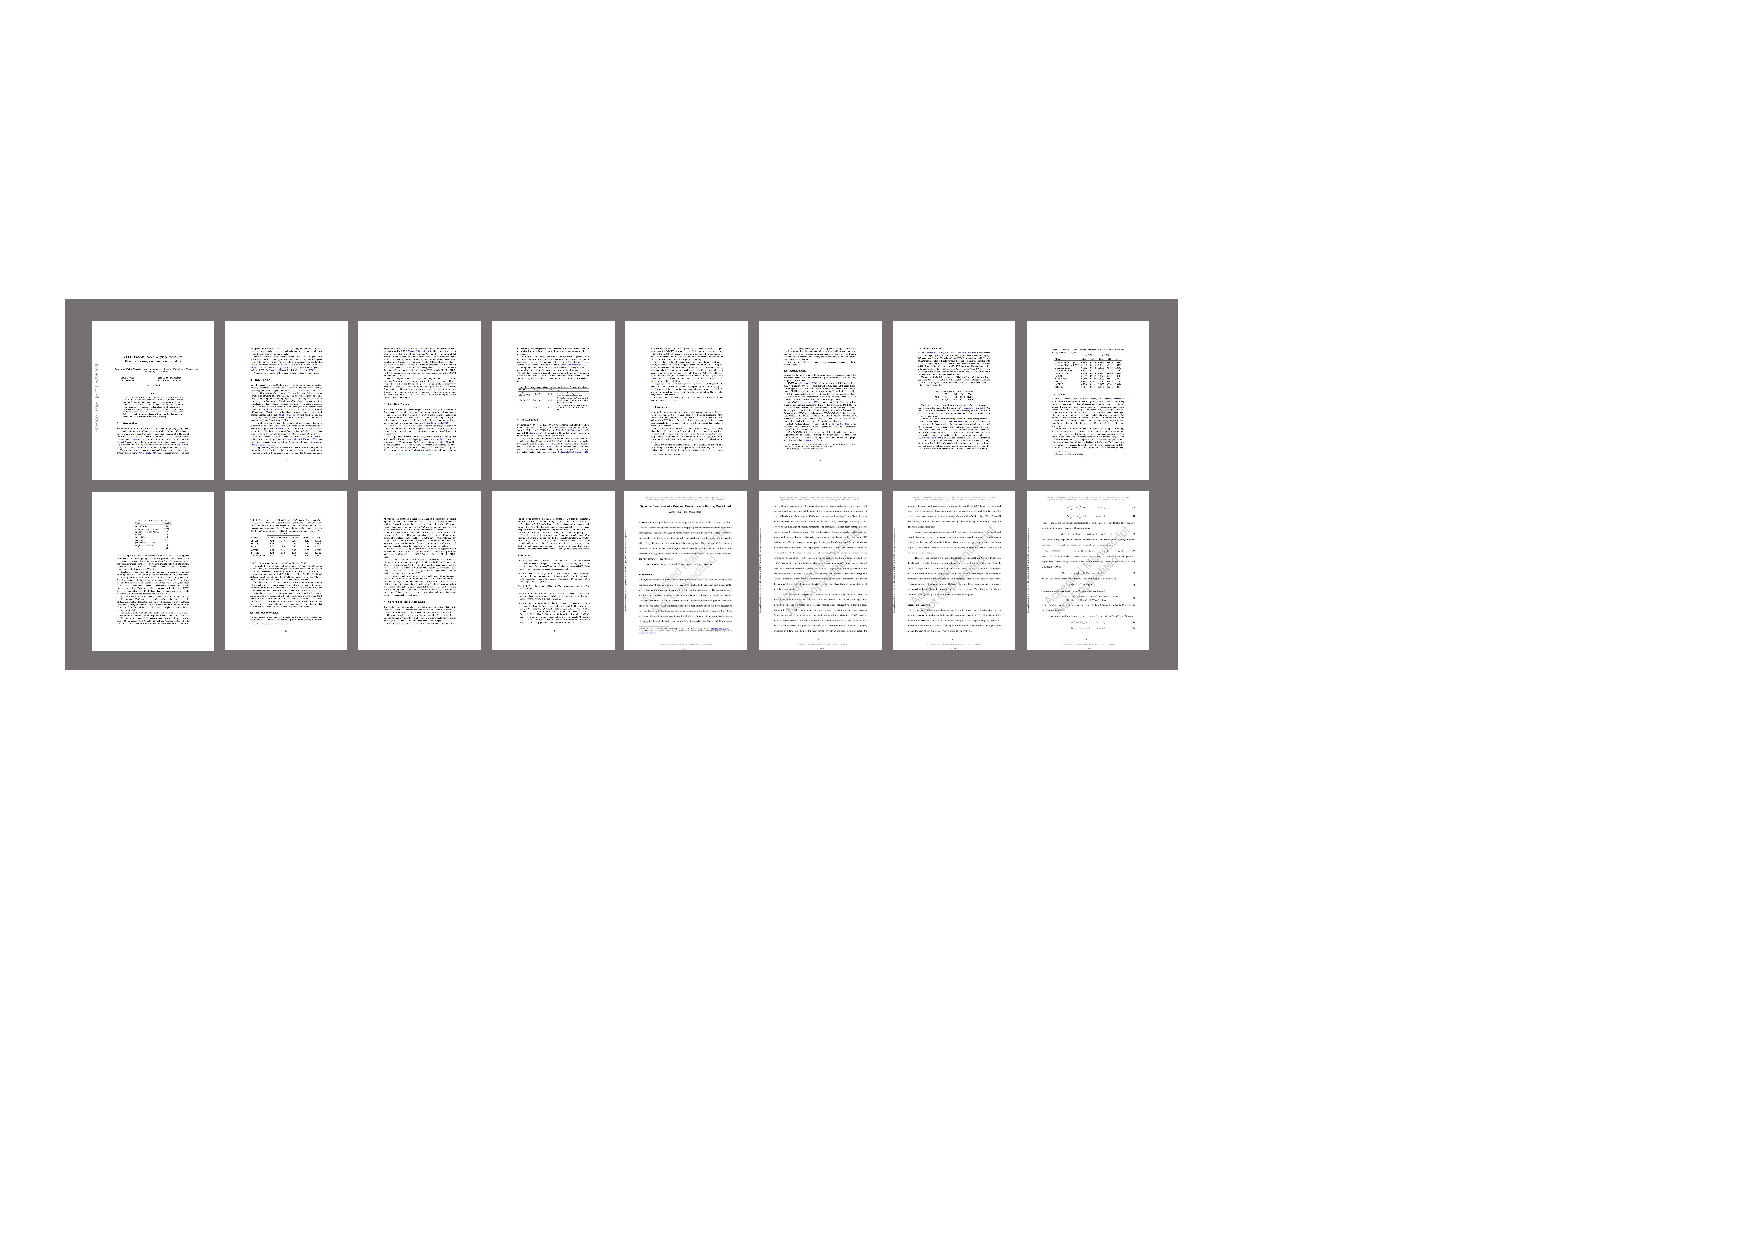
\includegraphics[width=\linewidth]{figure/multi-image_format.pdf}}
    \caption{
    \textbf{An example of multi-image format document.} Each page of the document is rendered as an image.
    }
    \label{fig:multi-image}
\end{figure*}

\begin{table*}[t]
\centering
\renewcommand\arraystretch{0.2}
\begin{tabular}{l|c|l|l}
\toprule
Datasets          & \#QA  & Image Types                          & Tasks \\ 
\midrule
MP-DocVQA~\cite{tito2023mpdocvqa}         & 46K   & PDF Documents 
& VQA \\
\midrule
DUDE~\cite{van2023document}              & 41K   & PDF Documents 
& \makecell[tl]{VQA} \\
\midrule
MP-DocStruct1M~\cite{hu2024mplugdocowl2}    & 1M    & PDF Documents 
& \makecell[tl]{Text Parsing, Text Lookup} \\
\midrule
MP-DocReason51K~\cite{hu2024mplugdocowl2}   & 51K   & \makecell[tl]{PDF Documents, \\ Infographics, Webpages, \\ Charts, Natural images}
& VQA \\
\midrule
DocGenome~\cite{xia2024docgenome}         & N/A   & \makecell[tl]{PDF Documents}
& \makecell[tl]{Layout Detection, Document Transformation} \\
\midrule
\dataname (ours)  & 758K  & \makecell[tl]{PDF documents, \\ Charts, Tables} 
& \makecell[tl]{VQA, Abstract Writing, Paper Titling, \\ Caption Writing, Experiment Writing, \\ Translation, Review, Reply }    \\ 
\bottomrule
\end{tabular}
\caption{\textbf{Comparison with other document-level datasets. }}
\label{tab:addi_dataset_comparison}
\end{table*}



\begin{figure*}[t]
    \centering
    \small
    {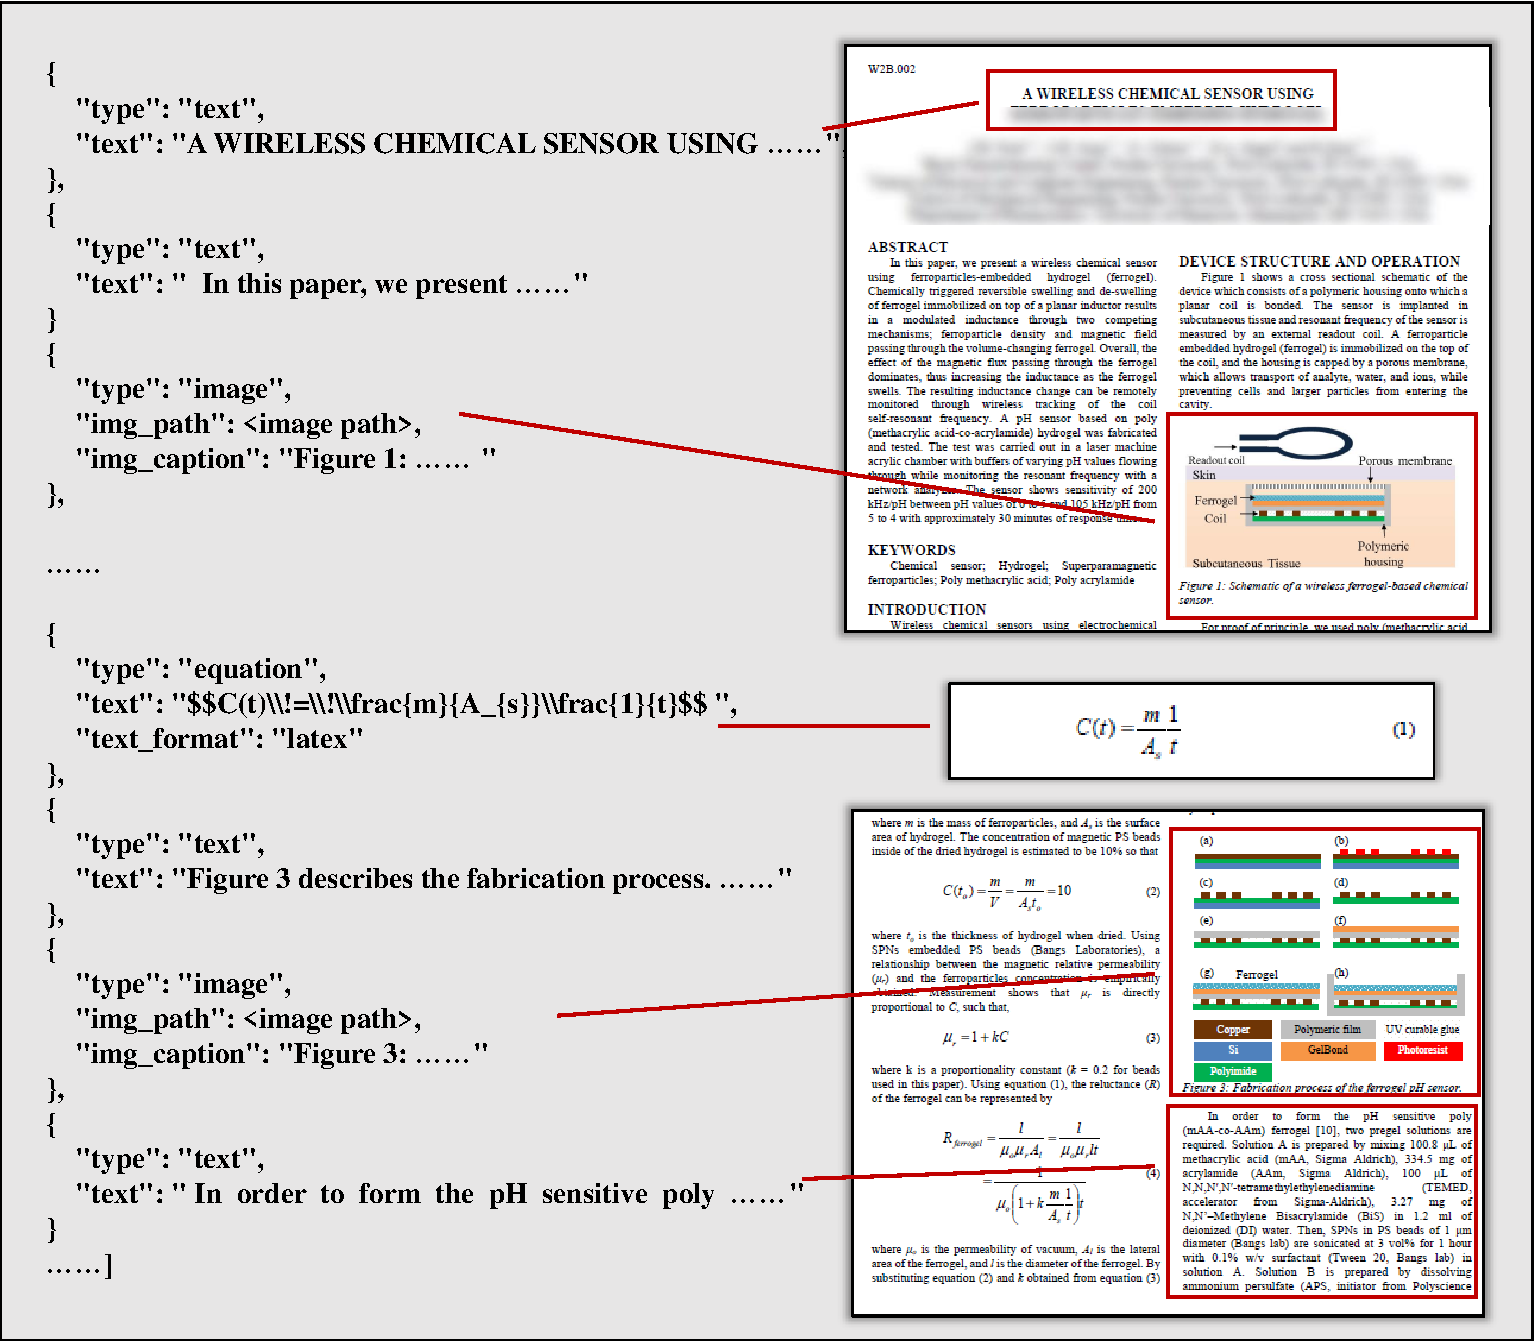
\includegraphics[width=.95\linewidth]{figure/interleaved_example.pdf}}
    \caption{
    \textbf{An example of interleaved text-image format document.} We capture the documents' textual content and construct them into interleaved images and text. 
    }
    \label{fig:interleaved-image_text}
\end{figure*}


\subsection{Image Types and Tasks Coverage}
We provide additional comparisons of \dataname with various document-level datasets in terms of image types and task coverage, as shown in Table~\ref{tab:addi_dataset_comparison}. Compared to these datasets, \dataname exhibits greater diversity in proxy tasks and ranks among the largest datasets in terms of QA pair count.



\subsection{Question-Answer Pairs Generation}
\noindent\textbf{Prompt.} The prompt used to generate question-answer pairs from GPT-4o is shown below.

\promptbox{Please read the paper and first check if this is an English paper. If it is not an English paper, don't do any other things. If it is an English paper, please design about 3 to 5 question-answer pairs based on the paper. All questions should require as much text as possible to answer and it is better to ask about the images in the papers. All images in the questions should be represented as the mentioned title in the paper like Figure 1/Figure 2 or Table 1/ Table 2 and they must be mentioned in the questions. The question should be specific enough that it can only be answered with the paper. The question should also be interesting and intellectual enough that a curious reader of the paper would ask about it. The answer of the QA pair must start with "According to the original text ......”, first give the relevant original text in the reference content, and then answer the question in detail. Please try to analyze the asked image in the answer. Please directly output a list of the QA pairs without any other outputs. Here is the paper: \\
<paper>
}

\noindent\textbf{Examples.} In Section~\ref{sec:data_engine}, we propose diverse question-answer formats tailored to data from different sources. To fully utilize the webpage structure of OpenReview, we develop tasks focused on review writing and replies within its review-reply framework. For Sci-Hub and Arxiv, we use their well-defined writing structures to create tasks such as writing and translating various sections. We provide examples of these various QA formats in Figure~\ref{fig:qa_example}.  

\noindent\textbf{Quality Evaluation.} The quality of \dataname is ensured through the following measures: 
(1) Human-Originated Data: QA pairs from OpenReview are derived from human-written discussions, providing high contextual quality.
(2) Structured Tasks: Tasks like abstract writing and paper titling are constructed based on document metadata, following deterministic rules to ensure reliability.
(3) Synthetic QA: We randomly sample and manually review 500 
training QA pairs across tasks and 498 of 500 (over 99\%) of the pairs were relevant. 

\begin{figure*}
  \centering
  \small
  \fbox{
    \parbox{.95\linewidth}{\texttt{\textbf{Review Writing} \\
    Question: Please review the following paper and provide a constructive critique. Focus on the methodology, results, and overall contributions, and highlight both strengths and areas for improvement. Your review should be detailed and insightful, offering suggestions for enhancing the research. Here is the paper: \\
    <paper>\\
    Answer: <review> \\ 
    \textbf{Reply Writing} \\
    Question: Given the following paper and its review, write a reply to address the feedback provided. Here is the paper:\\
    <paper>\\
    Here is the review:\\
    <review>\\
    Answer: <reply>\\ 
    \textbf{Abstract Writing} \\
    Question: Please read the full text of the following research paper and provide a concise summary in the form of an abstract. The summary should capture the main objectives, methods, results, and conclusions of the paper. Ensure that the abstract is clear, coherent, and informative for readers who have not read the full paper. Here is the paper:\\
    <paper w/o abstract>\\
    Answer: <abstract>\\
    \textbf{Paper Titling} \\
    Question: Based on the provided abstract or introduction of the research paper, please generate a concise and informative title that accurately reflects the main focus and contributions of the paper. The title should be engaging and clearly convey the essence of the research. Here is the abstract and introduction:\\
    <abstract> \\
    <introduction>\\
    Answer: <title>\\ 
    \textbf{Caption Writing} \\
    Question: The images or tables and their relative texts in a research paper are given interleaved as follows. Please write a caption for each image or table based on the relative texts provided. Here is the image:\\
    <image>\\
    Here is the relative text:\\
    <text>\\
    Answer: <caption>\\ 
    \textbf{Experiments Writing} \\
    Question: Please write the "Experiments" section based on the incomplete research paper provided. Ensure that the section is well-structured and includes the details of the Figures and tables. Here is the paper:\\
    <paper w/o experiments>\\
    Answer: <experiments section>\\ 
    \textbf{Translation} \\
    Question: Please read the full text of the following research paper and translate the Experiments/Abstract section into Chinese. Here is the paper:\\
    <paper> (Multi-Image format) \\
    Answer: <translation>\\ 
    \textbf{Multi-Turn QA (interleaved and rendered)} \\
    Question: Please read the full paper and answer the question. Here is the paper:\\
    <paper>\\
    Here is the question: <question> (generated)\\
    Answer: <answer> (generated)\\
    Question: <question> (generated)\\
    Answer: <answer> (generated)
    }}
  }
  \caption{\textbf{The examples of different formats of the QA pairs.} All tasks leverage the inherent structure of the documents.}
  \label{fig:qa_example}
\end{figure*}

\begin{table*}[t]
\centering
\setlength\tabcolsep{4pt}
\begin{tabular}{c|l|l|l}
\toprule
Layout    & Benchmark       & Description                             & Metric                                                                                      \\
\midrule
\multirow{3}{*}{Single-Page} & DocVQA~\cite{mathew2021docvqa}          & VQA on documents.                       & ANLS                                          \\
                             & ChartVQA~\cite{masry2022chartqa}        & VQA on charts.                          & Relaxed EM                                    \\
                             & InfoVQA~\cite{mathew2022infographicvqa}         & VQA on infographics.                    & ANLS                                          \\
\midrule
\multirow{5}{*}{Multi-Page}  & MP-DocVQA~\cite{tito2023mpdocvqa}       & VQA on multi-page documents.            & ANLS                                          \\
                             & MMLongBench-Doc~\cite{ma2024mmlong} & VQA on super-long PDF documents.        & Accuracy, F1 Score                            \\
                             & \multirow{3}{*}[3ex]{DocGenome~\cite{xia2024docgenome}}  & \multirow{3}{*}[3ex]{VQA on multi-page scientific documents.} & Classification Acc, \\
                             &                                  &                                                          & Title ED, Abstract ED, \\
                             &                                  &                                                          & Single-Page Acc,   Multi-Page Acc \\
\midrule
Interleaved                  & MM-NIAH~\cite{wang2024mmniah}         & VQA on natural texts or images.         & Accuracy   \\ 
\bottomrule
\end{tabular}
\caption{\textbf{Evaluation benchmarks and metrics for document understanding.}
This table summarizes key benchmarks used in document understanding tasks across three layout types: single-page, multi-page, and interleaved. 
}
\label{tab:benchmark_metrics}
\end{table*}

\section{Evaluation Details}

\subsection{Benchmark Metrics}


We report the metrics of benchmarks used in the evaluation in Table~\ref{tab:benchmark_metrics}. 
For DocVQA~\cite{mathew2021docvqa}, InfoVQA~\cite{mathew2022infographicvqa}, and MP-DocVQA~\cite{tito2023mpdocvqa}, we employ ANLS to evaluate the similarity between model responses and ground truth answers, while ChartQA~\cite{masry2022chartqa} uses Relaxed Exact Match (Relaxed EM). For open-ended QA tasks in MMLongbench-Doc~\cite{ma2024mmlong} and DocGenome~\cite{xia2024docgenome}, we utilize GPT-4o to assess the correctness of answers and calculate GPT Accuracy. Other tasks in DocGenome follow their official evaluation metrics.

\subsection{Evaluation Settings}

\textbf{For single-page benchmarks} such as DocVQA, ChartQA, and InfoVQA, we conduct the evaluation using a unified prompt as follows:

\promptbox{<image> \\ 
<question> \\ 
Answer the question using a single word or phrase.}


\noindent\textbf{For multi-page benchmarks}, we discuss them case by case. We employed image concatenation for multi-page VQA benchmarks like MP-DocVQA, MMLongBench-Doc, and DocGenome to reduce the excessive input patches. Adjacent pages were vertically concatenated into a single image, with a maximum total image count limit of 18.

(1) For MPDocVQA, we use the prompt for a $N$ concatenated page document as follows:

\promptbox{Image-1: <concat-page 1> \\ 
Image-2: <concat-page 2> \\ 
... \\ 
Image-N: <concat-page N> \\ 
<question> \\
Answer the question using a single word or phrase.
}

(2) For MMLongBench-Doc and DocGenome, we use the official prompt in their open-sourced code base for response generation and extract the correctness of the answer using GPT-4o.

(3) For MM-NIAH, we use the original interleaved data format and calculate the accuracy by their official judgment function.

\noindent\textbf{Evaluation of LLMs on Multimodal Document Benchmarks.}
We utilized the InternVL2-8B as the OCR model to extract text from each image of the document, followed by post-processing to remove redundant responses. The text extraction prompt is as follows:

\promptbox{Image-1: <image> \\
Please extract the text from Image-1, while retaining as much of the original formatting and structured information (such as headings, paragraphs, lists, tables, charts, etc.) as possible. If the document is not in PDF format, provide a caption for Image-1. Present the extracted information directly without additional explanations.
}

We concatenated the extracted texts to replace the original document images for the language models:
\vspace{-2ex}
\promptbox{Page 1: \\
<text 1>  \\
Page 2: \\
<text 2> \\
... \\
Page N: \\
<text N>
}

For the image-text interleaved data, we replaced the images with the captions as the input.


\noindent\textbf{Implementation Details of Multimodel RAG.}
VisRAG~\cite{yu2024visrag} uses their proposed retrieval model VisRet to calculate scores for each image and text segment based on the query. InternVL-RAG~\cite{wang2024needle} utilizes InternVL-14B, a CLIP-like model, to compute the similarity between images and text. For multi-paged VQA benchmarks, we select the top-3 retrieved documents for generation. For interleaved VQA, we choose up to 8K tokens for the generation.


\section{Training Details}
\subsection{Hyperparameters}
We report the models and training hyperparameters of \modelname-2B and \modelname-8B in Table~\ref{tab:hyperparam}.

\begin{table}[h]
\centering
\small
\setlength\tabcolsep{3.6pt}
\begin{tabular}{c|l|cc}
\toprule
\multicolumn{2}{c|}{Settings}              & \modelname-2B     & \modelname-8B             \\
\midrule
\multirow{2}{*}{\rotatebox{90}{Model}}     & ViT               & InternViT-300M      & InternViT-300M \\
                                           & LLM    & InternLM2-1.8B & InternLM2.5-7B \\

\midrule
\multirow{11}{*}{\rotatebox{90}{Training Hyperparameters}} & Tile Resolution   & \multicolumn{2}{c}{448}                                  \\
                                           & Batch Size        & \multicolumn{2}{c}{128}                                  \\
                                           & Optimizer         & \multicolumn{2}{c}{AdamW}                                \\
                                           & Learning Rate     & \multicolumn{2}{c}{1.00E-05}                             \\
                                           & Warmup Ratio      & \multicolumn{2}{c}{0.03}                                   \\
                                           & LR Scheduler      & \multicolumn{2}{c}{Cosine}                               \\
                                           & Weight Decay      & 0.01                & 0.05           \\
                                           & ViT Drop Path     & \multicolumn{2}{c}{0.1}                                  \\
                                           & Max Tile Number   & \multicolumn{2}{c}{24}                                   \\
                                           & Image Threshold   & \multicolumn{2}{c}{48}                                   \\
                                           & Token Threshold    & \multicolumn{2}{c}{32K}                                  \\
                                           & Epochs   & \multicolumn{2}{c}{1}              \\
\bottomrule
\end{tabular}
\caption{\textbf{Training settings and hyperparameters for \modelname models.} Key configurations for \modelname-2B and \modelname-8B, including model architectures and training parameters.}
\label{tab:hyperparam}
\end{table}

\subsection{Multimodal Packed Dataset}

In this section, we provide a detailed description of our packing algorithm. The main workflow is outlined in Algorithm \ref{alg:packed_dataset}. Specifically, our algorithm constructs the packed dataset by combining individual samples drawn from the original dataset. The packing operation involves four steps:

(1) \textbf{Check Sample:} Given an individual sample, we first verify whether the number of images exceeds the image threshold $T_i$ or the number of tokens exceeds the token threshold $T_t$. If either condition is met, the sample is truncated into $N$ parts. The first $N-1$ parts contain exactly $T_i$ images or $T_t$ tokens and are immediately added to the output. The remaining part is passed to the subsequent steps for further processing.

(2) \textbf{Find Buffer:} For the remaining part of the sample, we attempt to find a suitable buffer from the buffer list to pack it together with the sample. The combined result must not exceed the thresholds $T_i$ for images or $T_t$ for tokens, while maximizing the total number of images and tokens in the packed sample. To speed up this process, the buffer list is organized as a priority queue.

(3) \textbf{Pack Samples:} The given sample and the selected buffer are packed together. Notably, during the training process, each token can only attend to other tokens within the same original sample. Tokens from other samples packed together remain inaccessible.

(4) \textbf{Maintain Buffer List:} After generating a packed sample, we check if its number of images or tokens meets the specified thresholds. If so, the sample is added to the output; otherwise, it is reinserted into the buffer list for potential future packing.
Note that we omit numerous edge cases for brevity.

\begin{algorithm}
	\caption{Multimodal Packed Dataset} 
	\label{alg:packed_dataset} 

    \KwIn{Dataset $\mathcal{D}$, buffer list $\mathcal{B}$, Token Threshold $T_t$, Image Threshold $T_i$}
    \KwOut{Packed Dataset $\mathcal{D}_\text{packed}$}

    \ForEach{data\_sample $d$ in $\mathcal{D}$}{

        $b  \gets \texttt{find\_buffer}(d, B)$ 

        $b_{p} \gets \texttt{pack}(d, b)$

        \If{$b_{p}$ \text{contains more than} $T_i$ \text{images or} $T_t$ \text{tokens}}{
            \texttt{yield} $b_{packed}$
        }
        \Else{
            $\texttt{insert}(b_{packed}, B)$
        }
    }

\end{algorithm}


\section{Qualitative Examples}

In this section, we show a series of qualitative examples to illustrate the effectiveness of our \modelname in handling complex multi-page documents. Each figure highlights a specific capability of the model in addressing various tasks.

Figure~\ref{fig:good_sample1} demonstrates the model's ability to accurately retrieve relevant information from a multi-page document, showcasing its capability to perform robust cross-page retrieval tasks.

In Figure~\ref{fig:good_sample2}, we illustrate the model's proficiency in performing backward queries, where context must be traced across pages in reverse order to locate relevant content.

Figure~\ref{fig:good_sample3} highlights the consistency of answers when the model is queried across multiple pages. This example demonstrates that the model maintains coherence and accuracy even when information is distributed across different parts of the document.

Figure~\ref{fig:good_sample4} presents an example of counting across pages, showcasing the model's ability to integrate numerical information from disparate locations in a document. 

Lastly, Figure~\ref{fig:good_sample5} demonstrates the model's capability to pinpoint specific information within a designated section of a super-long document, emphasizing its fine-grained retrieval capabilities.

These examples collectively highlight the robustness and adaptability of our approach in understanding and processing multi-page documents effectively.

\section{Limitations}
The objective of \dataname is to develop a large-scale, multi-task, multimodal document-level QA dataset that efficiently trains MLLMs for document understanding. Sourced primarily from open academic platforms, the dataset focuses on tasks like multi-page QA, reasoning, and translation, with some academic-specific tasks such as titling and summarization. 
A key limitation of \dataname is its current domain restriction to academic documents. We plan to expand the dataset’s coverage to a broader range of document types and enhance the generalizability of proxy tasks, ensuring wider applicability across diverse domains.

\begin{figure*}[]
    \centering
    {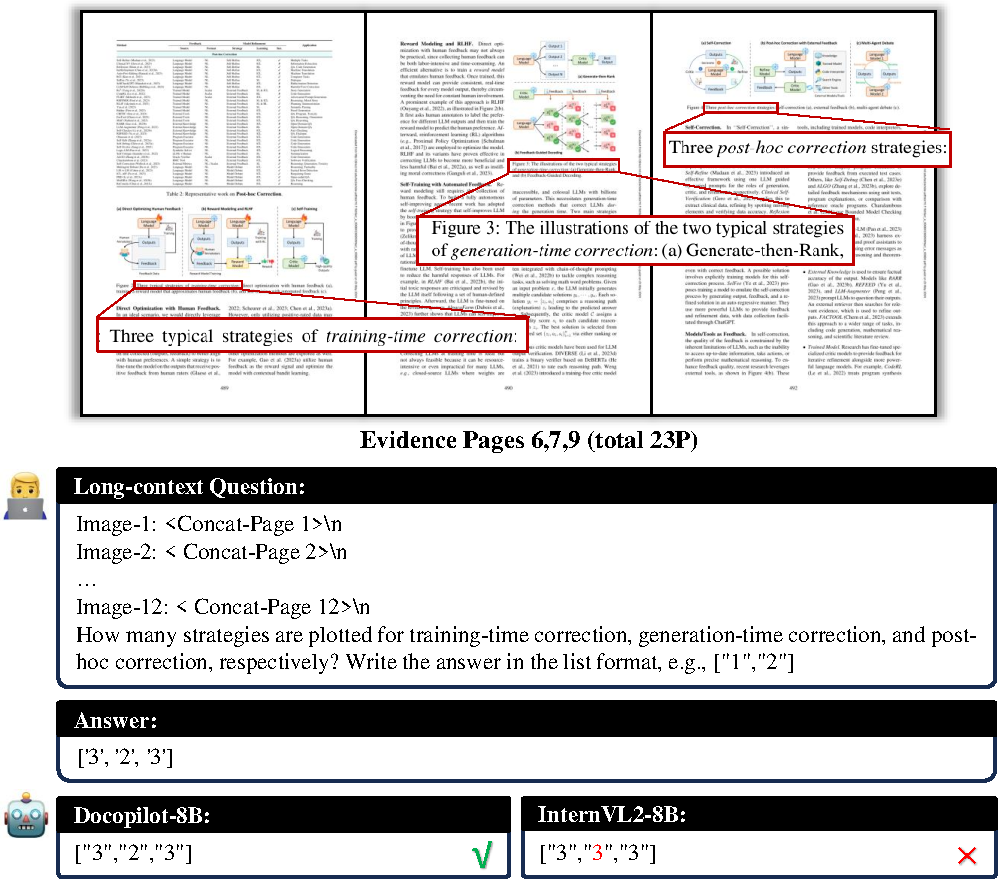
\includegraphics[width=0.65\linewidth]{figure/sample1.pdf}}
    \caption{\textbf{A qualitative example of retrieval in a multi-page document.}}
    \label{fig:good_sample1}
\end{figure*}

\begin{figure*}[]
    \centering
    {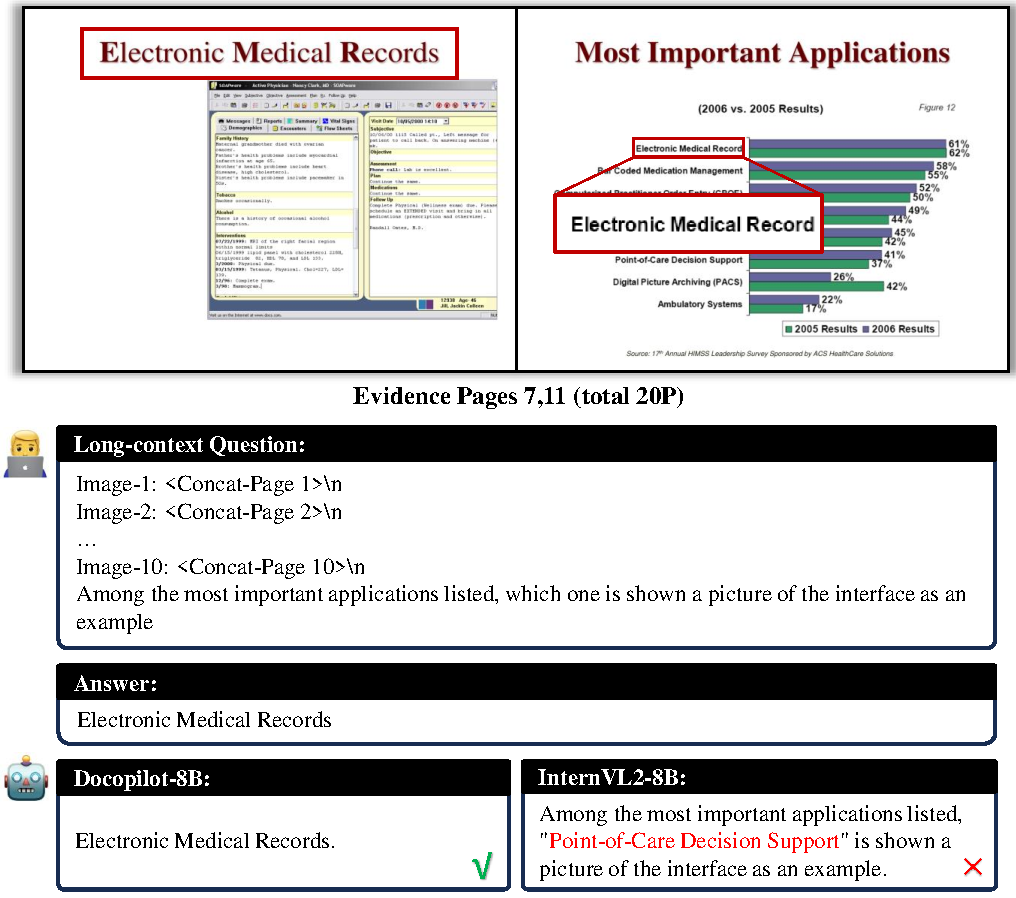
\includegraphics[width=0.65\linewidth]{figure/sample2.pdf}}
    \caption{\textbf{A qualitative example of backward query in a multi-page document.}}
    \label{fig:good_sample2}
\end{figure*}

\begin{figure*}[]
    \centering
    {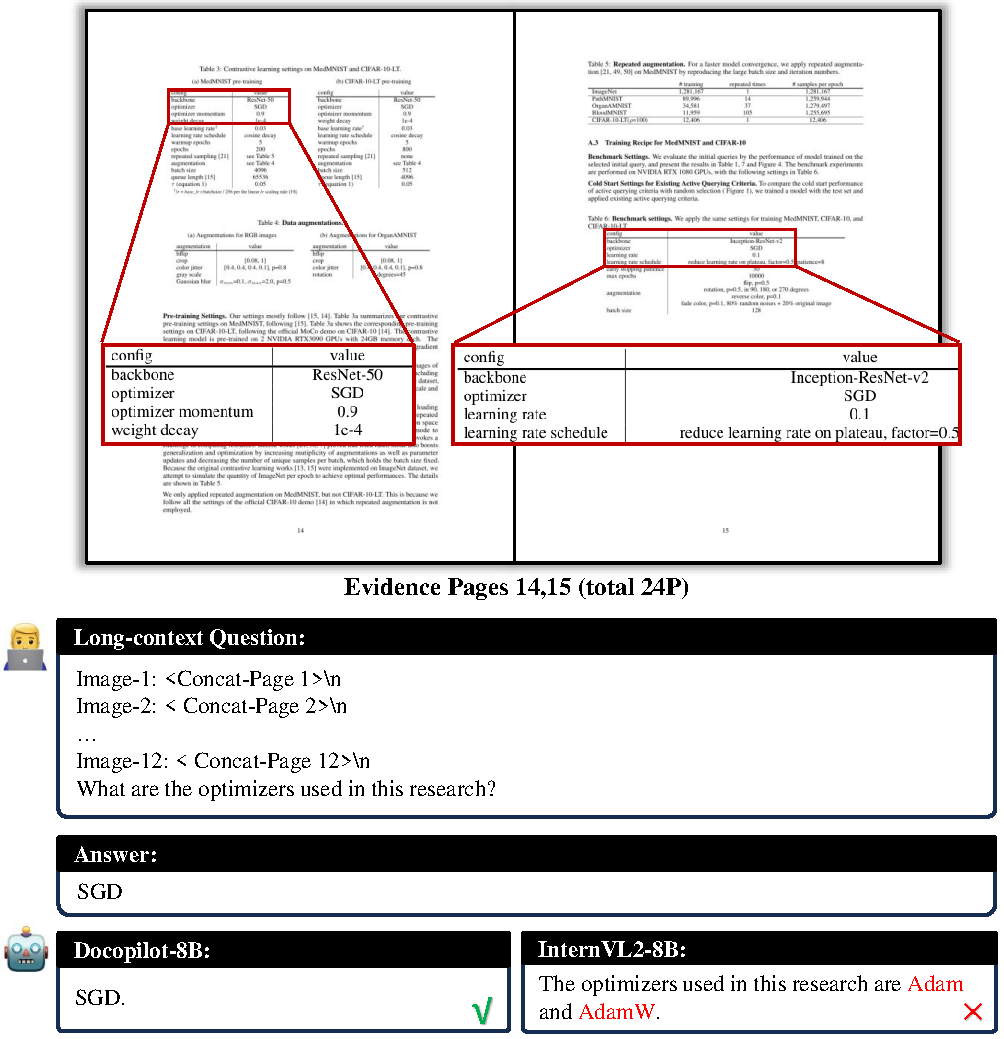
\includegraphics[width=0.6\linewidth]{figure/sample3.pdf}}
    \caption{\textbf{A qualitative example of consistency of answers in multi pages.}}
    \label{fig:good_sample3}
\end{figure*}

\begin{figure*}[]
    \centering
    {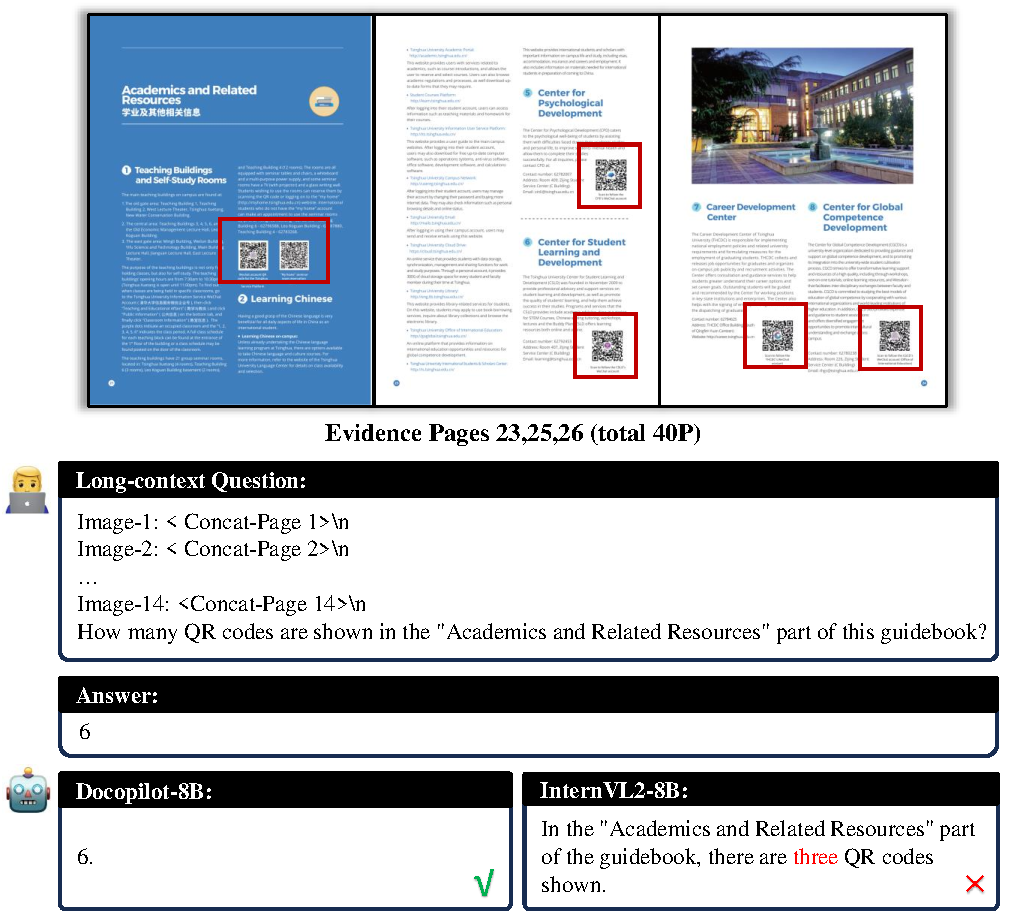
\includegraphics[width=0.6\linewidth]{figure/sample4.pdf}}
    \caption{\textbf{A qualitative example of counting across pages.}}
    \label{fig:good_sample4}
\end{figure*}

\begin{figure*}[t]
    \centering
    {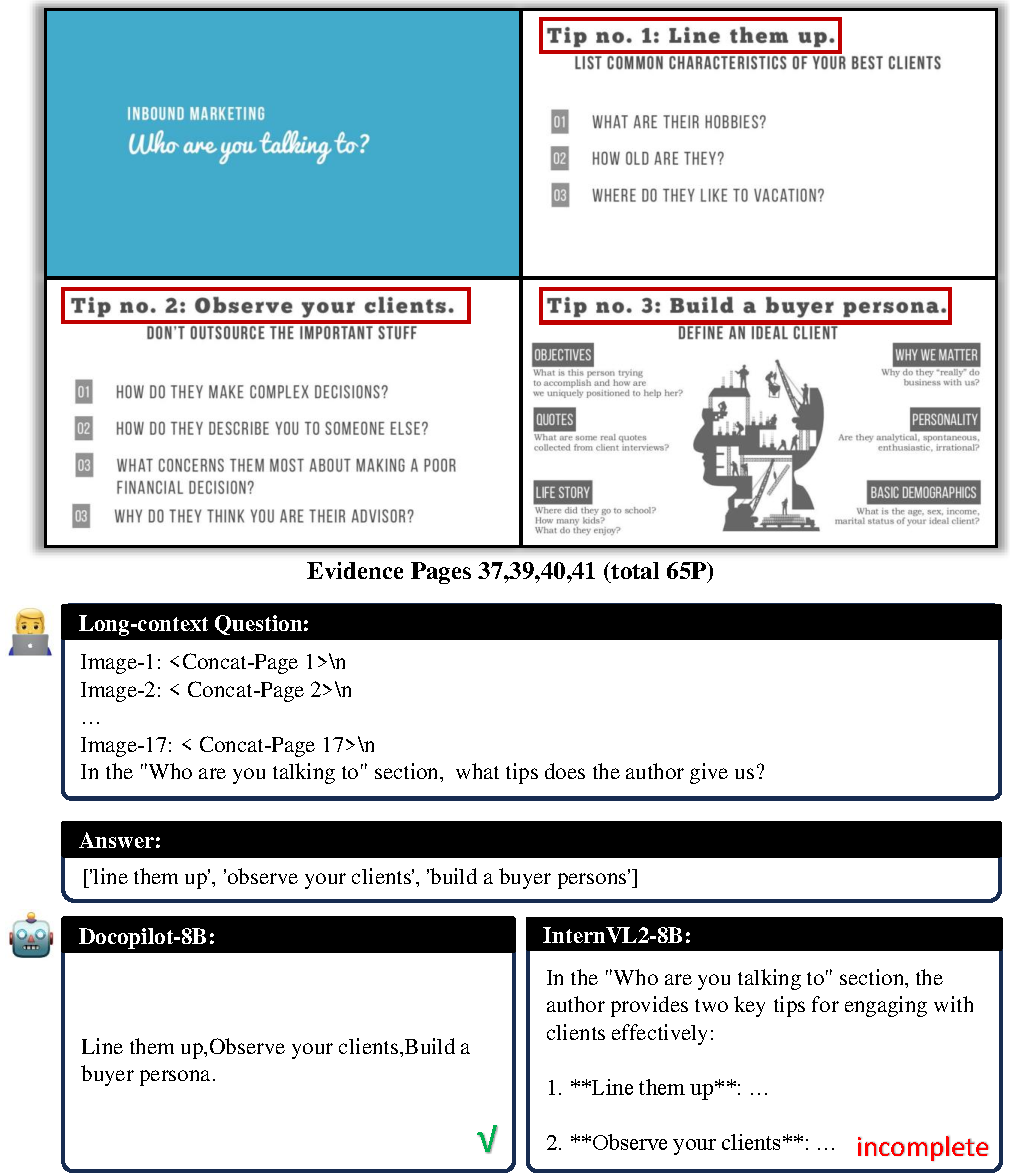
\includegraphics[width=0.6\linewidth]{figure/sample5.pdf}}
    \caption{\textbf{A qualitative example of retrieval in a specific section of a super-long document.}}
    \label{fig:good_sample5}
\end{figure*}
